\documentclass{article}
\usepackage[utf8]{inputenc}
\usepackage{graphicx}
\usepackage{subcaption}
\usepackage{amsmath}
\usepackage{setspace}
\usepackage[
  backend=biber,
  style=apa,
  citestyle=apa
]{biblatex}
\usepackage{geometry}
\geometry{
 a4paper,
 total={150mm,237mm},
 left=30mm,
 top=30mm,
 }

\renewcommand{\baselinestretch}{1.5} 
\addbibresource{references.bib}

\title{DAGs with Applications to Macroeconomic Timeseries}
\author{Emmet Hall-Hoffarth}
\date{July 2020}

\begin{document}

\maketitle

\abstract{DAGs are a type of graphical model that can under some conditions allow for causal inferences to be made from observational data. Despite the clear value of a such a tool in economic applications, little empirical work has been done in this area. Therefore, this paper aims to address this by considering the application of DAGs to simulated and real macroeconomic timeseries data. The results indicate that DAGs perform reasonably well at identifying the expected causal pathways in simulated and real data when variables are not subject to selection and are small in number relative to the sample size, but may struggle otherwise.}

\section{Introduction}

Directed Acyclical Graphs (DAGs) \parencite{pearl1995causal} are a form of graphical model that are particularly useful for modelling causal probabilistic relationships. This framework has many benefits, chief among them that under some conditions one can infer a DAG and thus an causal model of a Data Generating Process (DGP) directly from observed data. This property opens the door for numerous useful economic applications. However, Imbens (\citeyear{imbens2019potential}) notes a lack of concrete empirical examples demonstrating the usefulness of this methodology in the field of economics, citing some potential drawbacks and pitfalls. Therefore, the purpose of this paper is to investigate the applicability of DAGs in economic applications, and to consider an empirical example in the field of macroeconomics. 

The application involves modelling simulated data from well-known macroeconomic DSGE models, as well as real macroeconomic timeseries. This application has a number of appealing properties. Firstly, because in a simulation the true DGP is known, it will be possible to precisely evaluate to what extent it is possible to identify the true underlying structure of the data using DAGs. Furthermore, in this controlled environment it is possible to ensure that the assumptions required by DAGs are satisfied, and therefore it provides a fair way to evaluate their applicability. Finally, these models are the central building blocks of modern macroeconomics and therefore provide a very relevant example of how DAGs can be applied in economics.

The remainder of this paper will be organised as follows. Section 2 will provide a review of the relevant literature on both DAGs and DSGE models, relating the two to each other where appropriate. Section 3 will introduce the methodology, that is, the specific implementation of DAGs used in the empirical study. Section 4 will discuss the data used in the empirical study. Section 5 will present the results of the empirical study. Section 6 will conclude and discuss avenues for future research.

\section{Liturature Review}

\subsection{DAGs}

The fundamental assumption of a DAG is that the underlying DGP of some observed data can be represented as a Directed Acyclical Graph (DAG). Figure \ref{dag1} shows an example of a DAG. Each of the variables in the data forms a node in the graph, and these nodes are connected by arcs. The direction of each of the arcs represents the direction of causality in the sense of conditional probability. For example, if we observe the DAG $B \rightarrow A$, then A's distribution is conditional on B, whereas B is distributed $i.i.d.$ In economic language the analogous interpretation is that B is exogenous (in every possible sense) while A is endogenous to or determined by B. As the name DAG implies, arcs are assumed to not create any cycles in the graph. For a given node, the set of nodes which have an arc pointing into that node are known as that node's parents, and the set of nodes that have an arc pointing into them from that node are known as that node's children. A root node is a node that has no arcs leading into itself, and a leaf node is a node that has not arcs leading out of itself.

\begin{figure}
  \centering
  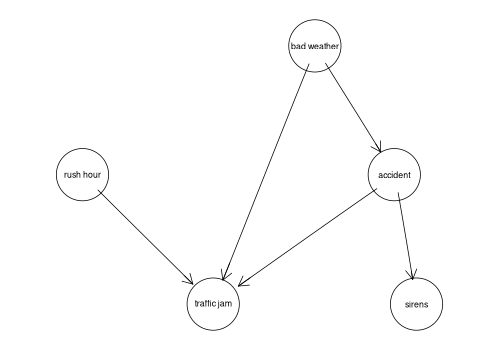
\includegraphics[width=0.8\textwidth]{images/trafficjam.png}
  \caption{An example of a simple DAG \parencite{traffic_jam}}
  \label{dag1}
\end{figure}

Each arc represents a conditional probability relationship. As a result DAGs satisfy the causal markov assumption such that the distribution of each variable depends only on its parents in the graph. For example, in figure \ref{dag1}: 

\begin{equation}
  \label{eq1}
  p(sirens | data) = p(sirens | accident)
\end{equation}

These conditional probabilities are abstract in the sense that they could be treated as either discrete or continuous, and any distributional assumption of choice could be applied to them. While much of the literature surrounding DAGs focuses on the discrete case, in many economic applications continuous variables are the primary concern. This is possible as long as we are willing to make some distributional assumption about the nature of the conditional probability. The most common assumption here (and fortunately the most natural economic one), is that the conditional distributions follow a multivariate normal distribution of the conditioning variables. This is implies that conditional distributions are linear functions of conditioning variables with Gaussian errors, which is exactly the assumptions of simple, small-sample OLS regressions common in econometrics. Such models are sometimes known as "Gaussian Bayesian Networks." (GBN) For example:

\begin{equation}
  \label{eq2}
  sirens|data = sirens|accident = \alpha + \beta accident + \epsilon, \space \epsilon \sim N(0, \sigma^2)
\end{equation}

Therefore, this technique is "non-parametric" in the sense that we do not make any assumptions about which underlying relationships exist between variables (indeed, this is what we hope the model will tell us). However, we do make a distributional assumption about the conditional distributions.

When fully specified, a GBN consists of a system of linear equations that defines the joint distribution of the data. Because of the properties of the normal distribution, this means that we can express a GBN as a single joint normal distribution over the data, where the DAG specifies the exact restrictions that are imposed on the covariance matrix. In order to enhance clarity of exposition, in this paper all DAGs are assumed to be Gaussian unless otherwise specified. The primary benefit of this simplification is the fact that uncorrelatedness implies independence, although it is by no means necessary, and many of the same results hold for arbitrary distributional assumptions.

\subsubsection{Identification of Causal Effects}

This section considers the situations in which an observationally constructed DAG can correctly identify causal effects. Pearl (\citeyear{pearl2009causality}) defines a sufficient assumption as the "back-door criterion." A set of observed variables $z$ is said to satisfy the back-door criterion relative to $x$ and $y$ if:

\begin{enumerate}
  \item no node in $z$ is a decendent of $x$ \label{bd1}
  \item $z$ blocks every path between $x$ and $y$ that contains an arrow into $x$ \label{bd2}
\end{enumerate}

Here a path is any combination of arcs connecting one node to another (regardless of direction), a backdoor path is a path that is not directed, and a path between $x$ and $y$ is blocked if $x$ and $y$ are independent in the DAG given $z$. Intuitively, this is the concept in economics commonly described as unconfoundedness. Although more general, it implies in particular that even if there are variables that are relevant to the true DGP that are unobserved, the DAG can still consistently estimate the causal effect of $x$ on $y$ as long as $x$ and $y$ have no common, unobserved causes (confounders). In particular, this identifying assumption allows for the causal effect of $x$ on $y$ to be observed, even if there is some unobserved variable $u$ that intermediates (lies along) the causal path. This is profound in many economic applications where models assume that some unobservable function intermediates the relationships between observed variables. For example, a (unobservable) utility function intermediates the path between the observable determinants of demand such as price and preference ordering, and the quantity purchased. In this context, the back-door criterion implies that even if the true DGP contains a utility function which is unobservable to and even ignored by the observational DAG it is still possible correctly identify the causal effect of the demand determinants on the quantity purchased as long as all relevant determinants of the utility function are observed. The back-door criterion implies that complex functions that intermediate the relationship between observables are \textit{emergent} in the model without being explicitly assumed.

Of course, the backdoor critierion is limited in the same way as any unconfoundedness identification strategy: it is difficult to argue and in many cases implausible that there is no backdoor path (unobserved confounder) between the causal variables of interest. However, DAGs can also consistently identify a causal effect if it satisfies the "front-door criterion." A set of variables $z$ is said to satisfy the front-door criterion relative to variables $x$ and $y$ if it satisfies the following three assumptions \parencite{pearl2009causality}:

\begin{enumerate}
  \item $z$ blocks all directed paths from $x$ to $y$
  \item there are no unblocked back-door paths from $x$ to $z$
  \item all back-door paths from $z$ to $y$ are blocked by $x$
\end{enumerate}

\begin{figure}
  \centering
  \begin{subfigure}{0.45\textwidth}
    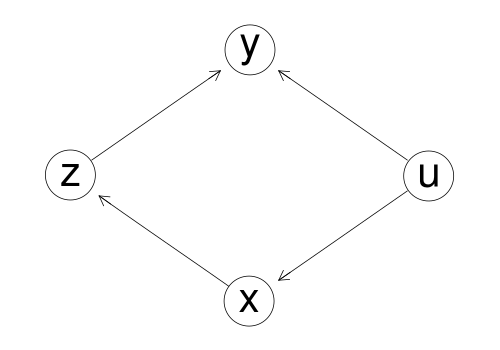
\includegraphics[width=\linewidth]{images/frontdoor.png} 
    \caption{Front-door criterion}
    \label{dag8_fd}
  \end{subfigure}
  %
  \begin{subfigure}{0.45\textwidth}
    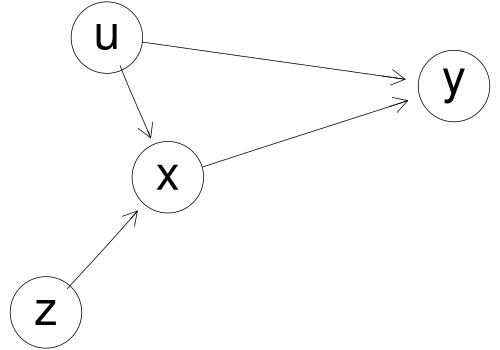
\includegraphics[width=\linewidth]{images/iv.png}
    \caption{Instrumental variables}
    \label{dag8_iv}
  \end{subfigure}
\end{figure}

The front-door criterion is demonstrated by figure \ref{dag8_fd}. Intuitively, what this allow s for is a sort of reverse instrumental variables identification where the instrument $z$ intermediates the causal path from $x$ to $y$ instead of being a parent/determinant of $x$. The assumptions here are similar in scope to those made in instrumental variables. The first assumption is akin to the exclusion restriction, the second exogeneity, and the third relevance.

Both the back-door and front-door criterion make strong assumptions about unobserved variables, which raises questions about their applicability. However, this problem is hardly specific to DAGs. Empirical economists are well acquainted with the difficulty of making arguments of unconfoundedness that are also required by many traditional econometric techniques, such as the exogeneity assumption required for instrumental variables. Because DAGs are an easily scalable machine learning technique they can add a sort of "brute force" tool to the empirical economics toolbox. This technique allows for causal inference by appeal to high-dimensional data sets where assumptions such as uncondoundedness are more plausible rather than the clever arguments and insights usually required by econometric models over a small number of observed variables.

\subsubsection{Identification of DAGs} \label{stability}

We now consider the assumptions which must be made of a DGP for it to be correctly modelled by as a DAG. \citeauthor{pearl2009causality} (\citeyear{pearl2009causality}) identifies the relevant condition as \textit{stability} or \textit{faithfulness}. Under this condition there exists a minimal structure of the true DGP which is a DAG. Faithfulness is the assumption that the conditional independence relationships in the DGP are robust to changes in the perturbations to the value of parameters. An equivalent statement of the condition is that a DAG is \textit{faithful} to a given DGP if the statistical independences in the DGP are exactly those implied by the DAG \parencite{spirtes2000causation}. This assumption is only violated if some causal effects exactly cancel out, resulting in no observed correlation between casually connected variables. \citeauthor{pearl2009causality} (\citeyear{pearl2009causality}) provides the following example demonstrating how faithfulness can fail. Consider the following model: $z = \beta_{zx} x + \epsilon_x$, $ y = \beta_{yx} x + \beta_{yz} z + \epsilon_y$. If we impose the parameter restriction $\beta_{yx} = -\beta_{yz}\beta_{zx}$ then $x$ and $y$ are independent. However, this independence relationship is not robust to perturbations of the model parameters and is therefore not stable in the relevant sense. 

A sufficient condition for faithfulness is that the DGP parameters are jointly continuous over the parameter space \parencite{steel2006homogeneity}, or equivalently, that the matrix of DGP parameters is of full rank. This is because under this condition, specific combinations of parameters which result in the cancelation of causal effects have a probability of 0 of occuring, even if they are possible. If we believe that the true DGP of the macroeconomy is DSGE model, which itself is faithfully represented by a DAG, then this condition is unlikely to be met. DSGE models impose many cross-equation restrictions on parameters that effectively reduce the rank of the parameter matrix. Unfortunately this condition will not allow us to guarantee that DSGE models satisfy the faithfulness assumption. However, if when considering real macroeconomic data we put aside the assumption that the true DGP is a DSGE model, it does not seem \textit{a priori} unreasonable that the parameter relating, for example, capital and output, and the parameter relating consumption and technology vary independently in different populations. Regardless, this condition is merely sufficient, not necessary, and so it does not rule out that DSGE models can be faithfully represented by DAGs. 

In another approach to failures of faithfulness, \citeauthor{steel2006homogeneity} (\citeyear{steel2006homogeneity}) notes that such failures or near-failures (that is near-zero statistical dependence despite clear causal pathways) are likely occur when parameters are both subject to \textit{selection} and \textit{homogeneity}. In this context, selection means that parameters are at least partially determined by an economic agent. The suggestion is that if the path of a policy variable $z$ is specifically designed as a function of $x$ to counteract the causal effect of $x$ on some outcome $y$, then it is reasonable to believe that little or no correlation will be observed between $x$ and $y$ despite a clear causal pathway between them. If parameters are assumed to be come from some distribution with different draws for each population, then homogeneity is the statement that there is little exogenous variation in those parameter values, that is variation outside of the variation caused by selection. If \textit{both} selection and homogeneity occur, failure or near-failure of faithfulness is likely to occur. Within the context of macroeconomics, this seems likely to be the case when considering interest rates and the actions of central banks. Assuming the interest rate is set according to a Taylor (\citeyear{taylor1993discretion}) rule, the parameters of that rule are chosen with the specific intent and canceling the causal effect of inflationary shocks on output and minimizing exogenous variation. This example seems to satisfy both selection and homogeneity. On the other hand, many parameters of the macroeconomy, in particular real ones, are plausibly not prone to this type of selection (for example, the autoregressive coefficient on an exogenous technology process). This distinction will be important when considering the empirical results in this paper.

\subsubsection{Estimation} \label{estimation}

There are two fundamental problems to solve when estimating a DAG. The first is known as "parameter learning," and the other "structure learning." Given a DAG as in Figure \ref{dag1}, the first task is simply to estimate the parameters of the network, such as $\alpha$ and $\beta$ in Equation \ref{eq2}. This is usually done via maximum likelihood, however, other "score" functions are available such as the Bayesian Information Criterion (BIC) \parencite{chen1998speaker}.

\begin{figure}
  \centering
  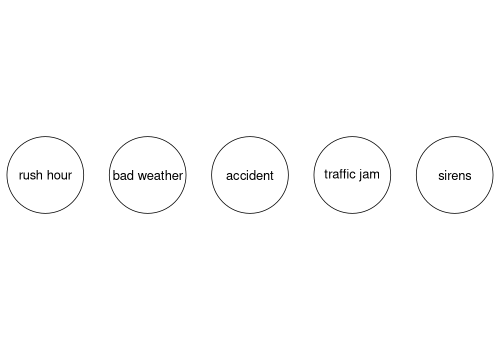
\includegraphics[width=0.8\textwidth]{images/trafficjam_unfit.png}
  \caption{A DAG before structure learning}
  \label{dag2}
\end{figure}

The second task, as demonstrated by Figure \ref{dag2} is that if we just start with some data it is not obvious which conditional probabilities to estimate in the first place. One way to do this is for the researcher to specify explicitly which conditional probabilities should be present in the graph, and simply fit the parameters of that graph. How this can be done in the context of DSGE models is discussed in Section \ref{dsge}. In this context however, doing so achieves little. This is equivalent to specifying a system of linear regressions to be estimated, probably based on some economic model that was developed by other means, and while this is then automatically encapsulated in a convenient, easily interpreted representation of the underlying assumptions, it seems nothing particularly novel would have been achieved. 

A more more exciting approach is to algorithmically learn the structure of the graph, that is to learn a structural model, directly from observed data. One "brute force" method to solving this problem is to compute the posterior likelihood of every possible network, however, this number is super-exponential in the number of variables such that it becomes very computationally expensive, very quickly \parencite{chickering1996learning}. As a response to this, many heuristic approximation techniques have been developed. These can be grouped into two categories: constraint-based and score-based structure learning algorithms \parencite{spirtes1991algorithm} \parencite{verma1991equivalence}. 

\begin{figure}
  \centering
  \begin{subfigure}{0.3\textwidth}
    \centering
    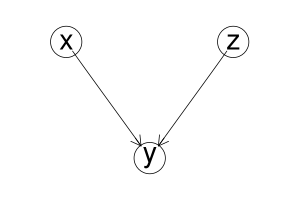
\includegraphics[width=\linewidth]{images/collider.png} 
    \small
    \begin{equation*}
      x = \epsilon_{x}
    \end{equation*}
    \begin{equation*}
      y = \beta_{yx} x + \beta_{yz} z + \epsilon_{y}
    \end{equation*}
    \begin{equation*}
      z = \epsilon_{z}
    \end{equation*}
    \caption{Collider}
    \label{collider}
  \end{subfigure}
  %
  \begin{subfigure}{0.3\textwidth}
    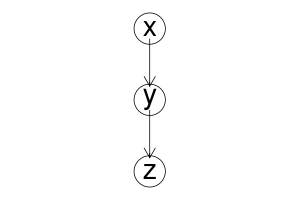
\includegraphics[width=\linewidth]{images/chain.png}
    \small
    \begin{equation*}
      x = \epsilon_{x}
    \end{equation*}
    \begin{equation*}
      y = \beta_{yx} x + \epsilon_{y}
    \end{equation*}
    \begin{equation*}
      z = \beta_{zy} y + \epsilon_{z}
    \end{equation*}
    \caption{Chain}
    \label{chain}
  \end{subfigure}
  %
  \begin{subfigure}{0.3\textwidth}
    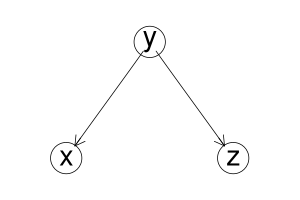
\includegraphics[width=\linewidth]{images/fork.png}
    \small
    \begin{equation*}
      x = \alpha_x + \beta_{xy} y + \epsilon_{x}
    \end{equation*}
    \begin{equation*}
      y = \epsilon_{y}
    \end{equation*}
    \begin{equation*}
      z = \beta_{zy} y + \epsilon_{z}
    \end{equation*}
    \caption{Fork}
    \label{fork}
  \end{subfigure}

  \caption{The three possible v-structures of a 3 node DAG. Error terms $\epsilon$ are all i.i.d. Gaussian shocks.}
  \label{dag5}
\end{figure}

Constraint-based algorithms rely on the fact that changing the direction of an arc changes the conditional independences implied by the graph, the presence of which can be tested for in the data. To see how the DAG assumptions can be sufficient to learn a causal model in this way, consider the example in figure \ref{dag5}. Suppose we have a graph with three nodes, such that no one node is completely independent from the other two (as this would make the graph trivial, and we could in any case rule out this case with an independence test). Furthermore, the graph cannot have all three possible arcs because it would either contain a cycle, or the third arc would imply a relationship which is redundant given the other two. Then the graph must have exactly two arcs. Given this, there are exactly three possible permutations of the network, which are the three shown in figure \ref{dag5}. These are known as the the three canonical "v-structures." \parencite{pearl2014probabilistic} These structures are partially identifiable from observational data because they imply different testable hypotheses about conditional independence. While the chain and fork imply that x and z are unconditionally dependent and only independent conditional on y, the collider implies exactly the opposite; that x and z are unconditionally independent and dependent conditional on y. Given some observed data we can easily test for the presence of conditional and unconditional independence under the assumption of joint-normality using a t-test on (partial) correations. The results of these tests can be used to rule out certain network structures which would be inconsistent with the observed data. Although for every set of three variables the network is only partially identifiable, full identification can (but will not always) be achieved when more variables are observed, by comparing overlapping triplets of variables and progressively reducing the set of network structures that are consistent both with the DAG assumptions and with the observed conditional independences. There are many that have been implemented using this general approach, the most popular of which is the PC algorithm first developed by \citeauthor{spirtes2000causation} (\citeyear{spirtes2000causation}). This algorithm has been shown to consistently estimate (as $n \rightarrow \infty$) the structure of the ground truth DAG of observed data under the assumptions of linear-Gaussian conditional probability functions, stability (as discussed in \ref{stability}), and structural complexity that does not grow too quickly relative to n \parencite{kalisch2007estimating}. 

Score-based methods as the name implies assign some score to every network based on its predictive accuracy and then use gradient-decent to identify the optimum network structure. There are a number of scoring functions and hill climbing algorithms that can be used to achieve this. A consistency result for the GES score-based algorithm is given in \citeauthor{chickering2002optimal} (\citeyear{chickering2002optimal}). The assumptions are slightly stronger than than that of the PC algorithm --- the number of variables must be fixed rather than growing slowly relative to n.

The major benefit of the constraint based method is that it directly utilises conditional independence as a primitive, which is the concept of causality that DAGs seek to identify. This is in contrast to score base methods, which effectively maximise the predictive accuracy of the model, and there is seemingly no guarantee that the most predictive model is the most likely causal explanation. In other words, despite the presence of large sample consistency results for both types of algorithms, it seems likely that small sample bias is more likely to be a problem for score-based methods. The major benefit of score based methods on the other hand is that they will always converge to a single fully directed graph as a solution whereas constraint based methods, because V-structures are only partially identifiable, may not be able to identify a unique solution. Instead, when the graph is only partially identifiable, the algorithm will return an undirected graph (CPDAG). The undirected arcs in a CPDAG could face either direction and the graph would still be consistent with both the DAG assumptions and the observed conditional independences. By permuting the two possible directions of each undirected arc we arrive at a set of graphs that are said to be "observationally equivalent." This is problematic because it is difficult or impossible to fit parameters to graphs that are not fully directed.  

Fortunately, these two methods can be combined into so called "hybrid" structure learning methods which use the strengths of both methods to counter the weaknesses of the other \parencite{scutari2014multiple} \parencite{friedman2013learning}. In this method the algorithm maximises a score function, but the number of parents that each node can have is restricted. The main benefit of this is a large gain computation efficiency because the search space is dramatically reduced, and theoretically it has the benefits of both constraint based and score based learning. However, while resulting the graph is always directed, it does not always correctly reflect the observed v-structures because it trades off constraint satisfaction and score maximisation. \citeauthor{nandy2018high} (\citeyear{nandy2018high}) gives an asymptotic consistency result for the ARGES hybrid learning algorithm.

\subsubsection{Causality and Inference} \label{cause}

Now that the mathematical underpinnings of DAGs have been introduced, it will be necessary to discuss the concept of causality that they employ, because it is somewhat different from what we are used to in economics. Most modern empirical work in economics utilises the potential outcomes causal framework \parencite{holland1986statistics}. In this framework a causal effect or treatment effect is defined as the difference between an outcome for an observational unit in the presence of a treatment $Y_i(1)$, and in the absence of the treatment $Y_i(0)$. This thinking is inspired by the medical and other physical sciences, where for example, the treatment effect of a medication on a patient's blood pressure is defined as the difference between the patient's blood pressure after taking the medication and \textit{what it would have been} if they had not taken the medication. Since in reality we can only ever observe one of these contingencies many statistical techniques have been developed that are able to consistently estimate this amount. Therefore, the potential outcomes framework can be said to make statements about counterfactuals, that is, the difference between outcomes in different states of the world.

The concept of causality that is relevant to DAGs is that of conditional independence. While this may seem unusual, this is actually akin to what is often assumed in macroeconomic theory, where every model has exogenous shocks that are the fundamental cause of the model dynamics. If we represent such macroeconomic models as DAGs these exogenous shocks would be the root nodes of the graph, because the root nodes of a DAG are assumed to be drawn independently of all other variables in the graph. In this framework the primary meaning of causality is exogeneity (that is in the literal sense, not being determined by what is observed), rather than treatment effects as in the potential outcomes framework. Since both of these concepts of causality (treatment effects and exogeneity) are commonly used in the field of economics one would like to believe that they are internally consistent, and indeed as I will argue in the remainder of this section, they are not incompatible. Indeed, DAGs are entirely consistent with potential outcomes and can be used to elicit counterfactuals / (average) treatment effects.

\begin{figure}
  \centering
  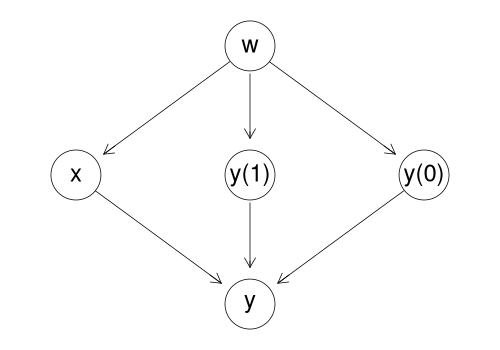
\includegraphics[width=0.8\textwidth]{images/potential_outcomes_dag.png}
  \caption{Potential Outcomes as a DAG}
  \label{dag6}
\end{figure}

Barr (\citeyear{barr2018causal}) gives an example of how the potential outcomes framework can be represented by a DAG, which is illustrated by figure \ref{dag6}. In this model, $w$ is a set of confounders, $x$ is the binary treatment of interest, $y(1)$ and $y(0)$ are the potential outcomes with and without the treatment respectively, and $y$ is $y(x)$. The fundamental assumption necessary for the consistent estimation of the average treatment effect here is that that given the confounders $w$ the treatment $x$ is independent of the potential outcomes. This is the assumption of unconfoundedness between the treatment and the treatment effects:
 
\begin{equation}
  x \perp \!\!\! \perp  (y(1), y(0)) | w
\end{equation}

In the graph, this assumption is illustrated by the fact that the only paths from $x$ to the potential outcomes are either through $y$, which is a collider which implies independence, or through $w$ which we have controlled for. This is an example of what Pearl (\citeyear{pearl2018book}) describes as the \textit{back-door criterion} which he identifies as a necessary conditions for DAGs to have a causal interpretation. This illustrates the deep conceptual similarities between these frameworks.

Furthermore, DAGs can be used to estimate counterfactual outcomes, using what Pearl (\citeyear{pearl2014probabilistic}) describes as \textit{do-calculus}. This uses the notation $P(y|do(x=\bar{x}))$. The difference between this and $P(y|x=\bar{x})$ is that $do(x=\bar{x})$ reflects an exogenous change in $x$ to $\bar{x}$, whereas $P(y|x=\bar{x})$ suggests that the model is in a state that would predict that the variable $x$ takes on the value $\bar{x}$. Under some conditions, computing $P(y|do(x=\bar{x}))$ can achieved by breaking the links of $x$ with its parents and setting it to $\bar{x}$, and then observing $y$ in the model. This is demonstrated by Figure \ref{dag3}. For example, consider Figure \ref{dag3}. Suppose for simplicity that all of the variables are binary (1 in the presence of the event, 0 otherwise). On the LHS of the diagram we have the model for observed values of all of the variables. On the RHS we intervene on $accident$. Notice that doing so breaks the link between $bad weather$ and $accident$. We can now estimate the causal treatment effect of an accident on the probability of a traffic jam given some values of $bad weather$ and $rush hour$ (in other words, all else equal) according to equation \ref{eq3}. This equation is very familiar, and is effectively the same as the calculation of an average treatment effect in the potential outcomes framework.

\begin{equation}
  \label{eq3}
  p(tj | bw = \bar{bw}, rh = \bar{rh}, do(a=1)) - p(tj | bw = \bar{bw}, rh = \bar{rh}, do(a=0))
\end{equation}

\begin{figure}

  \centering
  \begin{subfigure}{0.45\textwidth}
    \centering
    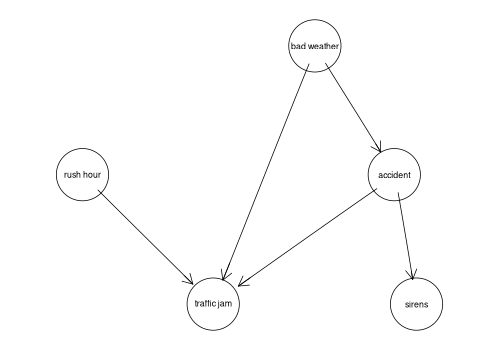
\includegraphics[width=\linewidth]{images/trafficjam.png} 
    \caption{No intervention}
  \end{subfigure}
  %
  \begin{subfigure}{0.05\textwidth}
    \centering
    $\rightarrow$
  \end{subfigure}
  %
  \begin{subfigure}{0.45\textwidth}
    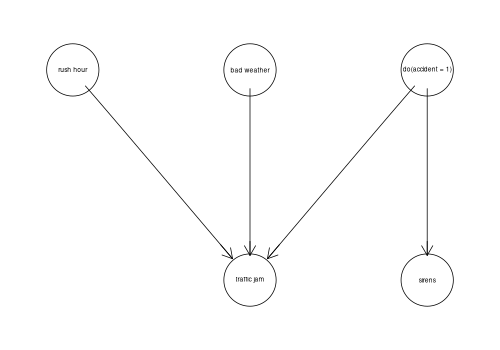
\includegraphics[width=\linewidth]{images/trafficjam_intervention.png}
    \caption{Intervention}
  \end{subfigure}

  \caption{An example of intervention}
  \label{dag3}
\end{figure}

In addition, there are other kinds of possible prediction exercises that we may be interested in with some economic interpretation. Since the model defines every endogenous variable as a (linear) function of the exogenous shocks it can be interpreted as a structural model of the data. Therefore, we might compute impulse response functions (IRFs) for each endogenous variable in the model to one or more shocks.

\subsubsection{Simultaneity} \label{simultaneity}

The concept of a DAG, while a powerful tool, is not a perfect model for all data. The strongest assumption is that it is directed. In many economic applications, while we may believe that some variables are truly exogenous such that they must be causes of movement in endogenous variables and not the other way around, we usually also assume that some or all of the endogenous variables are determined in general equilibrium, that is to say there is not necessarily a directionality to every relationship between endogenous variables. The problem of simultaneity is important, but there are ways which we can work with it in the DAG framework. I will propose two solutions to this problem: the first is that many relationships that we commonly think of as simultaneous have a mathematically equivalent fully directed model, and the second is that it is possible to relax the assumption that the graph is fully directed.

\begin{figure}

  \centering
  \begin{subfigure}{0.45\textwidth}
    \centering
    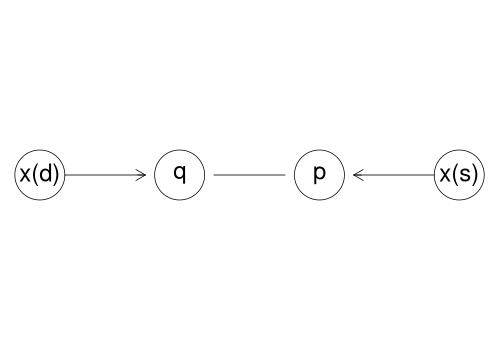
\includegraphics[width=\linewidth]{images/simultaneous.png} 
    \caption{Explcit simultaneity}
    \label{dag7_a}
  \end{subfigure}
  %
  \begin{subfigure}{0.05\textwidth}
    \centering
    $\iff$
  \end{subfigure}
  %
  \begin{subfigure}{0.45\textwidth}
    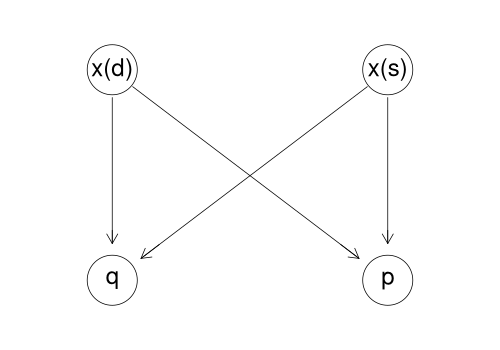
\includegraphics[width=\linewidth]{images/directed.png}
    \caption{Directed simultaneity}
    \label{dag7_b}
  \end{subfigure}

  \caption{An example of directing simultaneity}
  \label{dag7}
\end{figure}

In order to see why explicitly modelling simultaneity may not be necessary, consider figure \ref{dag7}, which is inspired by \citeauthor{imbens2019potential} (\citeyear{imbens2019potential}). Figure \ref{dag7_a} shows a simple model of supply and demand where quantity $q$ and price $p$ are determined simultaneously in the presence of demand shock $x(d)$ and supply shock $x(s)$. The relationship between quantity and price is simultaneous because changes in each one affect the other. However, the relationships implied by figure \ref{dag7_a} can just as well be represented by the fully directed graph in figure \ref{dag7_b}. To see this consider the following equations which are implied by figure \ref{dag7_a}:

\begin{equation}
  p = \alpha_p + \beta_{ps} x(s) + \beta_{pq} q + \epsilon_{p}
\end{equation}
\begin{equation}
  q = \alpha_q + \beta_{qd} x(d) + \beta_{qp} p + \epsilon_{q}
\end{equation}

By substituting $p$ into the equation for $q$ and vice versa it can be shown that this system of equations is equivalent to:

\begin{equation}
  \label{price_eq}
  p = \frac{1}{1-\beta_{pq}\beta_{qp}}[(\alpha_p + \beta_{pq} \alpha_q) + \beta_{ps} x(s) + \beta_{pq} \beta_{qd} x(d) + (\epsilon_p + \beta_{pq} \epsilon_q)]
\end{equation}
\begin{equation}
  \label{quantity_eq}
  q = \frac{1}{1-\beta_{qp}\beta_{pq}}[(\alpha_q + \beta_{qp} \alpha_p) + \beta_{qd} x(d) + \beta_{qp} \beta_{ps} x(s) + (\epsilon_q + \beta_{qp} \epsilon_p)]
\end{equation}

Which is (a version of) what is represented by figure \ref{dag7_b}. At this point I will note the relevance of the Lucas (\citeyear{lucas1976econometric}) critique. The model in \ref{dag7_b} is a reduced form estimation of the model in \ref{dag7_a}, and as such, it will be impossible to identify the policy parameters $\beta_{pq}$ and $\beta_{qp}$. In general, DAGs are a statistical technique that rely only on observed data, and therefore, they will not be immune to the Lucas critique. However, we \textit{can} identify the impact of exogenous shocks to the model. In the context of this example, this means that while the DAG cannot consistently estimate the supply and demand elasticities, it can consistently estimate the effect of a demand shock $x(d)$ or supply shock $x(s)$ on the equilibrium of the model. In the context of macroeconomic models we are often interested in computing IRFs which is the equilibrium effect of an exogenous shock to the model. This argument illustrates why even though we believe that many of the variables in these macroeconomic models are simultaneously determined, we can still estimate IRFs using DAGs. More generally, although DAGs might not be able to identify all structural parameters that economists might be interested in, they are nonetheless able to identify causal effects and there are likely to be many applications in which this is sufficient. For this reason, the discussion in the applications in this paper will focus on identifying the root nodes of a graph and their effects, while less emphasis will be placed on the relationships further down the causal tree.

However, it is also possible to explicitly model simultaneity in the context of graphical models. As discussed earlier, constraint based structure learning algorithms do not force a direction onto every arc, so it is entirely possible for structure learning to result in a Partially Directed Acyclical Graph (PDAG). Such models are known as hybrid networks or chain graphs, originally proposed by Wermuth and Lauritzen (\citeyear{wermuth1990substantive}). Recall that the DAG assumption can be characterised as a set of constraints on the covariance matrix of the joint normal distribution. In a hybrid network then there are no constraints on the partition of the covaraince matrix for the variables in the model that are assumed to be simultaneous. Note however, that while this approach may be more comfortable from the economic point of view it will still not immunise the model to the Lucas critique. Unfortunately, I was unable to find any convincing implementations which allow for hybrid networks. Therefore, all of the graphs that I use in my application are fully directed and used with appeal to the previous argument.

\subsection{DSGE Models} \label{dsge}

Having introduced DAGs as a modelling tool, this section will consider DSGE models and how they can be represented as DAGs. A the solution to a DSGE model is a state space model \parencite{hamilton1994state}, and therefore, all variables can be categorized as either state variables or control variables \parencite{fernandez2016solution}. Defined as generally as possible, state variables are the variables on whose past the model's current values depend, and control variables are the rest; their past is independent of the current values of the model. In the case of discrete time (the case considered in this paper) DSGE models have the Markov property, meaning that the current value of the states depends only on the history of the model in the previous period. State variables can be further categorized as either endogenous states (such as the capital stock) and exogenous states (such as the state of technology or productivity). As the name suggests, endogenous states are determined simultaneously (endogenously) with contemporanious controls in the model, however, their past is by definition exogenous and relevant to the determination of the current values of the model. Exogenous states, on the other hand, are exogenous in the sense that they are determined independently of any contemporanious variables in the model, and are thus determined entirely by the past of the model or any exogenous innovations (shocks) that might be present. The distinction between endogenous and exogenous states is subtle, but it is important here because the different implications about exogeneity will lead to a slightly different treatment in a DAG.

Given this definition it is straightforward to characterize the solution to a general DSGE model as a DAG. This is demonstrated by Figure \ref{dag11}. This expresses in graphical format all of the assertions in the previous paragraph about the solution to a DSGE model. There are a few important things to note here. Due to the Markov condition, it is only necessary to consider the first lag of the state variables, although this is done primarily for simplicity as this could easily be generalized. Models of this kind containing temporal data are sometimes known as Dynamic Bayesian networks \parencite{ghahramani1997learning}. Section \ref{simultaneity} argued that simultanous relationships can be represented by a DAG by simply expressing the (seemingly) endogenous variables as functions of the relevant exogenous variables. Here we use this to express the simultanously-determined contemporanious values of the controls and endogenous states as descendants of their exogenous determinants, namely, the lag of the endogenous states, and the current value of the exogenous states. Also note that the lag of control variables are completely detached from the rest of the graph.

\begin{figure}
  \centering
  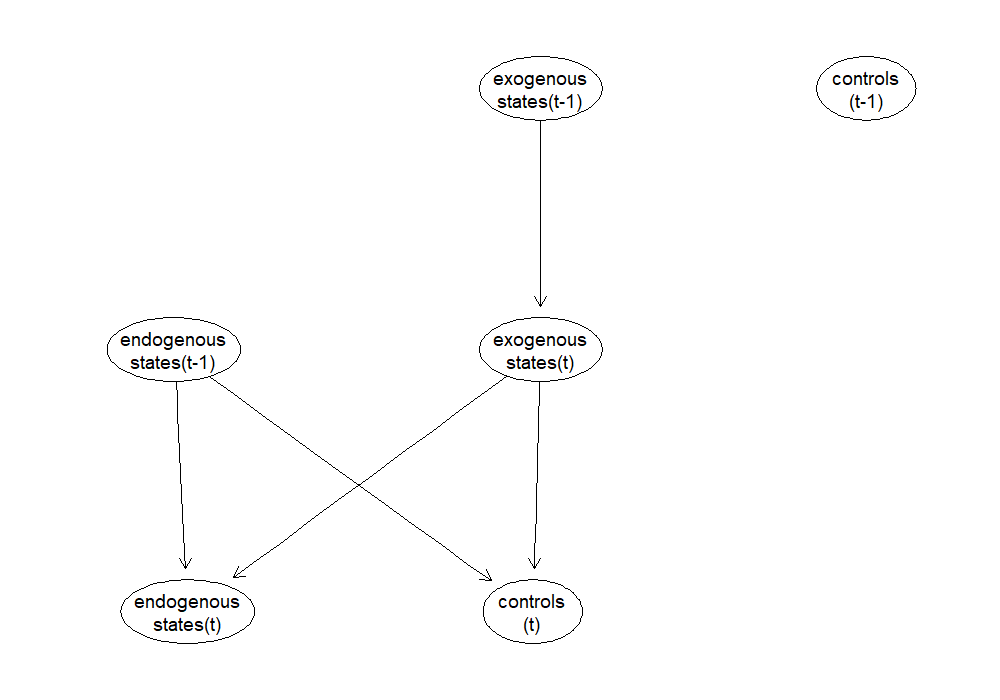
\includegraphics[width=0.8\textwidth]{images/dsge_dag.png}
  \caption{General solution to DSGE model as a DAG}
  \label{dag11}
\end{figure}

When data are simulated from a DSGE model the true endogenous states, exogenous states, and controls are known, and therefore it is straightforward to specify the solution to the model as a DAG as in Figure \ref{dag11}. In \ref{results} examples of this kind will be provided that further demonstrate that the solution to any DSGE model can be correctly specified as a DAG by using the DAG to reproduce the simualted IRFs. This DAG is the ground truth that structure learning algorithms seek to identify. Since we have asymptotic consistency results for all of the structure learning algorithms discussed in Section \ref{estimation}, we should be able to learn this ground truth as long as the relevant assumptions are satisfied. The assumptions of linear condtional probabilities and Gaussian innovations are satisified by the DSGE models employed here by construction. The assumption of faithfulness does not come for free and this may prove problematic for some models that will be considered here. Finally, the assumption that the sample size $n$ is large relative to the number of variables in the model can be easily satisfied in simulated data, but is a more important consideration in applications to real data. Therefore we will consider simulations with both large and small $n$.

\subsection{Related Modelling Techniques}

Having discussed how DSGE models and macroeconomic data more generally can be represented as DAGs this section will discuss how this approach relates to other econometric approaches which are common in the analysis of macroeconomic timeseries. It is possible to draw comparisions with both Structural Vector Autoregression (SVAR) and Autoregessive Distributed Lag (ADL) models, so these will be discussed in turn.

One of the most common and simplest econometric models for this type of data is the vector autoregression (VAR), which was popularized by \citeauthor{sims1980macroeconomics} (\citeyear{sims1980macroeconomics}). This method involves regressing a vector of outcomes $y_t$ on a matrix containing $k$ lags of $y$ in the form $y_t = [y_{t-1}, ..., y_{t-k}] \beta + \epsilon_t $. The primary concern with and limitation of this approach is that the estimated covaraince matrix $\epsilon_t$ is unrestricted, so the shocks contained within it are not mutually independent. Therefore, this model can not be used to estimate the effect of a truely exogenous shock on the dynamics of observed variables. In order to address this issue the model is transformed and an assumed causal ordering is imposed in the form of a Cholesky decomposition \parencite{sims1980macroeconomics}, which has the effect of making the errors of the estimated, transformed model mutally uncorrelated or \textit{structural}. Therefore, such models are known as SVARs. As noted by \citeauthor{demiralp2003searching} (\citeyear{demiralp2003searching}), in this context there is an equivallence between SVAR models and DAGs. This is because root nodes are assumed to be mutually uncorrelated, and as a result, any shocks to these will have a structural interpretation.

However, one key difference between a DAG in this context and a SVAR model is that the DAG allows for some variables to depend on contemporanious values of other variables. In particular, the endogenous states and controls depend contemporaniously on the exogenous states. In this sense the DAG is similar to an ADL model. When implementing an ADL model it is necessary for the researcher to choose which contemporanious variables to include as regressors, implicitly assuming that this regressors are at least predetermined relative to the outcomes of interest. 

The primary advantage of DAGs is the relatively weak assumptions they require. Both the SVAR and ADL models require the researcher to specify assumptions about the relative exogeneity of observable variables. These assumptions are themselves either derived from a similarly assumption-heavy model such as a DSGE model, or are entirely \textit{ad hoc}. There has been a long tradition within the field of economics including seminal papers by \citeauthor{lucas1976econometric} (\citeyear{lucas1976econometric}), \citeauthor{sims1980macroeconomics} (\citeyear{sims1980macroeconomics}), and \citeauthor{jorda2005estimation}, (\citeyear{jorda2005estimation}) criticising this type of model building. DAGs, along with structure learning algorithms provide an asymptotically consistent, agnostic, and data-driven alternative to models of this kind. 

\section{Methodology}

For the application in this paper I have used the "bnlearn" package \parencite{scutari2010bnlearn} for R. For the reasons outlined in section \ref{estimation} I used the implementation from this package of the hybrid "rsmax2" algorithm \parencite{spirtes2000causation}, with the PC algorithm as the structural constraint. This algorithm has a tuning hyperparamerter $\alpha$, which is the significance level of the t-test used in the PC algorithm. There is no general rule on the selection of this parameter, however, \citeauthor{kalisch2007estimating} notes that it should go to zero as $n$ goes to infinity. Therefore, results will be shown for a variety of choices of this parameter. Since the first lags of all variables in the model are added as nodes in the graph since it is not know \textit{a priori} which variables are controls or states. If structure learning succeeds in identifying the ground truth the lags of controls should be left disconnected from the rest of the graph, or at least have parameter values very close to 0. 

A number of general assumptions about DSGE solutions were encoded into the structure learning algorithm in order to reduce the size of the available search space and thus improve performance and accuracy. Firstly, no node that is a lag should have any parent nodes. A blacklist was therefore implemented in the PC algorithm to ensure this is the case in the resulting DAG. Secondly, an arc was manually added from the lag of each variable to its current value. At fist glance this would seem to contradict the fact that the lags of controls should be separate from the rest of the graph, however, during parameter estimation a slope parameter of 0 can be fit to these edges. Therefore this alteration does not remove the ground truth from the set of graphs the algorithm could potentially choose. Even though this alteration is theoretically allowable the primary justification for its inclusion is pragmatic. For example, consider a simpe DSGE model where an exogenous technology process follows an autoregressive process. If structure learning results in no edge between the lag and current value of technology, then any IRFs produced by this DAG would be highly inaccurate as the effect of a technology shock would disappear after only one period, even if the DAG otherwise does a good job of capturing the causal structure of the data.
Finally, the general DSGE DAG has an effective depth (the length of the longest directed path) of exactly three. Including this information in the structure learning algorithm would greatly reduce the size of the search space, and likely greatly improve structure learning performance. Unfortunately no implementation of the PC algorithm or any other structure learning algorithm that I was able to find is able to encode this kind of constraint, so this is left as a suggestion for future research. 

In order to evaluate the DAGs that are produced, I will consider two primary metrics. Firstly, I will consider the Structural Hamming Distance (SHD), which is defined as the number of edges that need to be added, removed, or reversed in order to transform the estimated DAG into the ground truth DAG \parencite{tsamardinos2006max}. This is a simple and effective measure of how close the algorithm has come to correctly identifying the underlying causal structure. Secondly I will use the estimated (and ground truth) DAGs to compute IRFs to a shock to one of the model's exogenous states ($z$). This is achieved according to the following process

\begin{enumerate}
  \item Set the values of all lags and exogenous states other than $z$ at time $t=0$ to 0.
  \item Set the value of $z$ at time $t=0$ to some external value, usually 1 standard deviation of the relevant shock.
  \item Impute the values of the remaining variables (the endogenous states and controls) implied by the DAG.
  \item Set lags in next time period to current values.
  \item Impute values implied by DAG in next period.
  \item Continue iteratively until period $T$ is reached.
\end{enumerate}

The purpose of this is to demonstrate that even when the structure of the estimated DAG does not appear to be entirely correct, it is still possible that it will reproduce the correct impulse responses, and this demonstrates how DAGs can be a useful small sample heuristic, even if the asymptotic properties do not apply.

\section{Data}

In order to demonstrate the capability of the DAG methodology empirically I will work with both simulated and real macroeconomic data. Using simulated data has a number of key advantages. Firstly, since the model that simulates the data is known it is possible to evaluate whether the structure learning has succeeded in identifying the ground truth DAG. Secondly, in this context it is possible to ensure to the greatest possible extent that the underlying assumptions of the structure learning algorithms, including linearity and normality are satisfied. Finally, since these models are central to modern macroeconomics it provides a controlled testing environment which is also arguably highly relevant to real data. On the other hand, using real data is an oppurtunity to demonstrate that DAGs are also a powerful heuristic tool that can be implemented outside of a rigorously controlled environment. The remainder of this section will discuss the various sources and general properties of the data used in this paper.

\subsection{Simulations}

In order to collect simulated data I consulted a github repository containing Dynare code to replicate a number of well known macroeconomic models \parencite{pfeifer2020}. In particular, I chose to model the baseline RBC model as a simple case and the \citeauthor{smets2007shocks} (\citeyear{smets2007shocks}) model for a more difficult and complex modelling challenge. I modified the simulation code slightly such that simulations would output a file containing $n$ observations of $i.i.d.$ draws of the exogenous shocks, and the associated observed values of the other variables in the model. This file was then used as the input for fitting DAGs.

\subsubsection{RBC}

\begin{table}
  \centering
  \begin{tabular}{|l|l|l|}
    \hline
    Symbol & Name & Type \\
    \hline
    $g$ & government spending & exogenous state \\
    $z$ & technology & exogenous state \\
    $k$ & capital & endogenous state \\
    $w$ & wage rate & control \\
    $r$ & return to capital & control \\
    $y$ & output & control \\
    $c$ & consumption & control \\
    $l$ & hours worked & control \\
    $i$ & investment & control \\ \cline{2-2}
    \hline
  \end{tabular}
  \caption{Description of Variables for RBC Model}
  \label{tab1}
\end{table}

The first model which I have chosen to evaluate is the baseline RBC model provided by \citeauthor{pfeifer2020} (\citeyear{pfeifer2020}). This model includes 11 variables which are summarized by Table \ref{tab1}. Using the default specification a sample of 100000 observations was generated, from which smaller subsamples are also considered. This model contains two exogenous state variables: technology ($z$) and government spending ($g$), and one endogeous state: capital ($k$). this model was chosen as it is one of the simplest DSGE models and provides a good baseline to demonstrate the effectiveness of DAGs in this context.

\subsubsection{Smets and Wouters (2007)}

\begin{table}
  \centering
  \begin{tabular}{|l|l|l|}
    \hline
    Symbol & Name & Type \\
    \hline
    $a$ & productivity & exogenous state \\
    $b$ & risk premium & exogenous state \\
    $g$ & government spending & exogenous state \\
    $qs$ & investment-specific technology & exogenous state \\
    $ms$ & monetary policy process & exogenous state \\
    $spinf$ & price markup process & exogenous state \\
    $sw$ & wage markwup process & exogenous state \\
    $cf$ & consumption (flex price economy) & endogenous state \\
    $invef$ & investment (flex price economy) & endogenous state \\
    $yf$ & output (flex price economy) & endogenous state \\
    $c$ & consumption & endogenous state \\
    $inve$ & investment & endogenous state \\
    $y$ & output & endogenous state \\
    $pinf$ & price inflation & endogenous state \\
    $w$ & real wage & endogenous state \\
    $r$ & nominal interest rate & endogenous state \\
    $kpf$ & capital stock (flex price economy) & endogenous state \\
    $kp$ & capital stock & endogenous state \\
    $zcapf$ & capital utilisation rate (flex price economy) & control \\
    $rkf$ & rental rate of capital (flex price economy) & control \\
    $kf$ & capital services (flex price economy) & control \\
    $pkf$ & real value of capital (flex price economy) & control \\
    $labf$ & labour supply (flex price economy) & control \\
    $wf$ & wage rate (flex price economy) & control \\
    $rrf$ & real interest rate (flex price economy) & control \\
    $mc$ & marginal cost & control \\
    $zcap$ & capital utilisation & control \\
    $rk$ & rental rate of capital & control \\
    $k$ & capital services & control \\
    $pk$ & real value of capital & control \\
    $lab$ & labour supply & control \\ \cline{2-2}
    \hline
  \end{tabular}
  \caption{Description of Variables for Smets and Wouters (2007) Model}
  \label{tab2}
\end{table}

The model from \citeauthor{smets2007shocks} (\citeyear{smets2007shocks}) on the other hand is a significantly larger and more complex model. This model was chosen because it is highly influential, and it represents the current state of the art in DSGE models. It also provides a more difficult modelling challenge to approach with DAGs. 

This model contains seven exogenous shocks: a productivity shock (ea), a risk premium shock (eb), a government expenditure shock (eg), an investment specific technology shock (eqs), a monetary policy shock (em), a price markup shock (epinf), and a wage markup shock (ew). These shocks each contribute (respectively) to an AR process of an exogenous state, whith the exception of wage and price inflation which follow an ARMA process, for a total of 7 exogenous states. Furthermore, the model has 11 endogenous states, while the remainder are controls.

\subsection{US Data}

\begin{table}
  \centering
  \begin{tabular}{|l|l|}
    \hline
    Symbol & Name \\
    \hline
    $pi$ & CPI Inflation \\
    $rm$ & Federal Funds Rate (Return to Money) \\
    $rb$ & 10 Year US Treasury Bond Yield (Return to Bonds)\\
    $g$ & (Real) Government Expenditure \\
    $y$ & (Real) GDP \\
    $i$ & (Real) Private Investment \\
    $w$ & Median (Real) Wage \\
    $n$ & Population \\
    $rk$ & Return to Capital \footnote{Estimated as average return to the NASDAQ over the relevant period} \\
    $z$ & Total Factor Productivity \\
    $u$ & Unemployment \\
    $l$ & Total Workforce \\
    $c$ & (Real) Personal Consumption \\\cline{2-2}
    \hline
  \end{tabular}
  \caption{Description of Variables for US Data}
  \label{tab3}
\end{table}

To provide an example of real macroeconomic timeseries, quarterly data from the US between years 1980-2005 were collected from FRED (\citeyear{fred2020data}) for 15 variables outlined in Table \ref{tab3}. All of the variables were detrended by taking the residuals of an estimated first order autoregression. Total factor productivity and capital stock were provided on an annual basis and were therefore interpolated quadratically. Full details of data preprocessing are availible on GitHub \parencite{hall2020git}.

\section{Results} \label{results}

\subsection{RBC}

\subsubsection{Structure Learning}

\begin{figure}

  \centering
  \begin{subfigure}{0.6\textwidth}
    \centering
    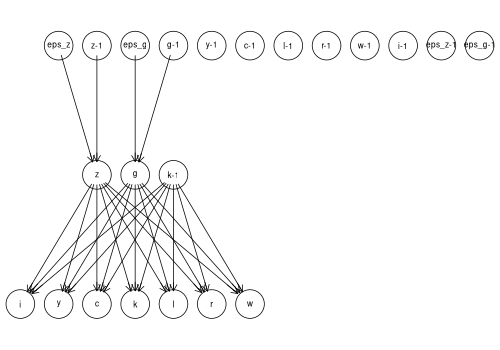
\includegraphics[width=\linewidth]{images/rbc_true_dag.png} 
    \caption{Ground Truth DAG}
    \label{gtdag}
  \end{subfigure}
  %
  \begin{subfigure}{0.6\textwidth}
    \centering  
    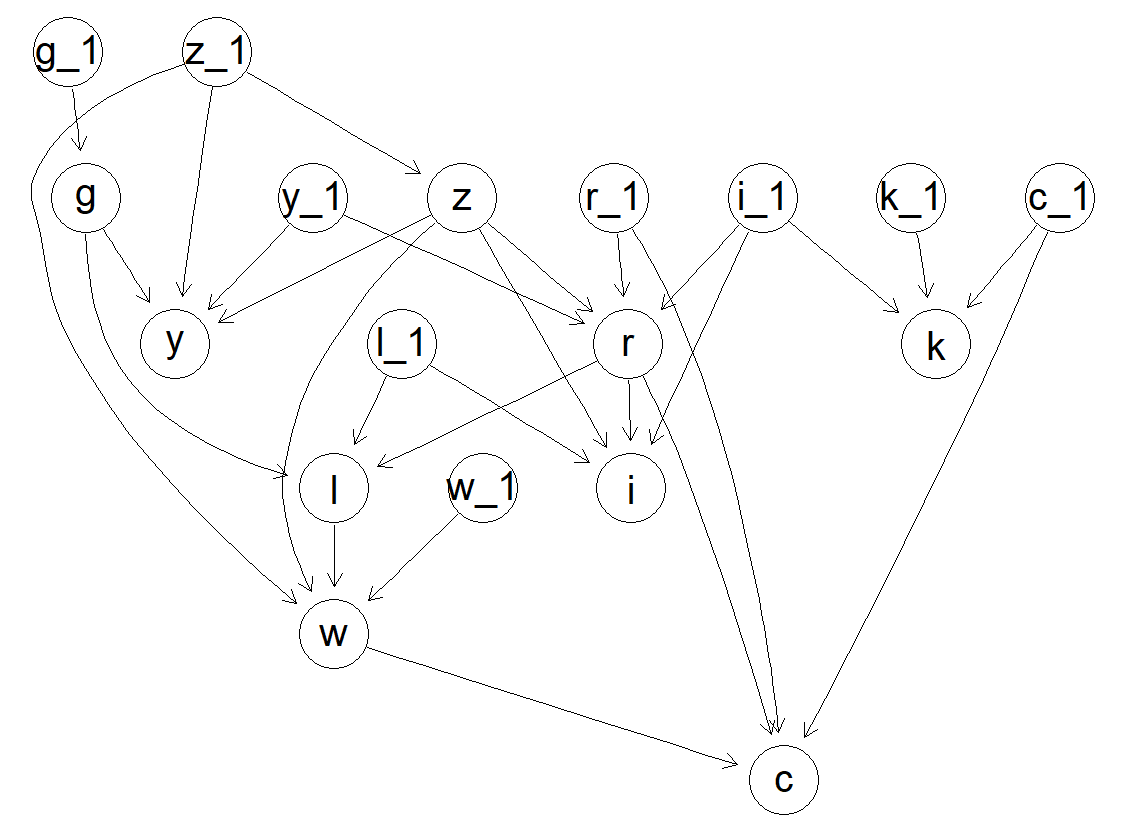
\includegraphics[width=\linewidth]{images/rbc_hybrid_structure.png}
    \caption{Hybrid DAG}
    \label{hdag}
  \end{subfigure}

  \caption{Structure of DAGs manually and algorithmically fit to RBC model data.}
  \label{rbcdags}
\end{figure}

Figure \ref{rbcdags} shows the ground truth DAG, as well as a DAG learned using the hybrid structure learning algorithm, with hypothesis test size $\alpha = 0.1$, and 100,000 observations. This graph has a SHD of 33. There are a few results to note here. Firstly, $z$ and $g$ are successfully identified as exogenous states, whereas $k$ is successfully identified as an endogenous state. On the other hand, no variable is identified as a control, as none of the autoregressive coefficients in the parameterized model fail to reject the null in a t-test at any reasonable significance level. Furthermore, although the graphs have similar number of overall edges (25 for the ground truth and 24 for the learned model), the learned model seems to be more sparse, in the sense that the average number of parents for each node is lower. One reason for this is that the learned model is much deeper than the ground truth. Here we can see how the ability to limit the depth of the resulting graph would likely improve results. 

\subsubsection{IRFs}

\begin{figure}

  \centering
  \begin{subfigure}{0.8\textwidth}
    \centering
    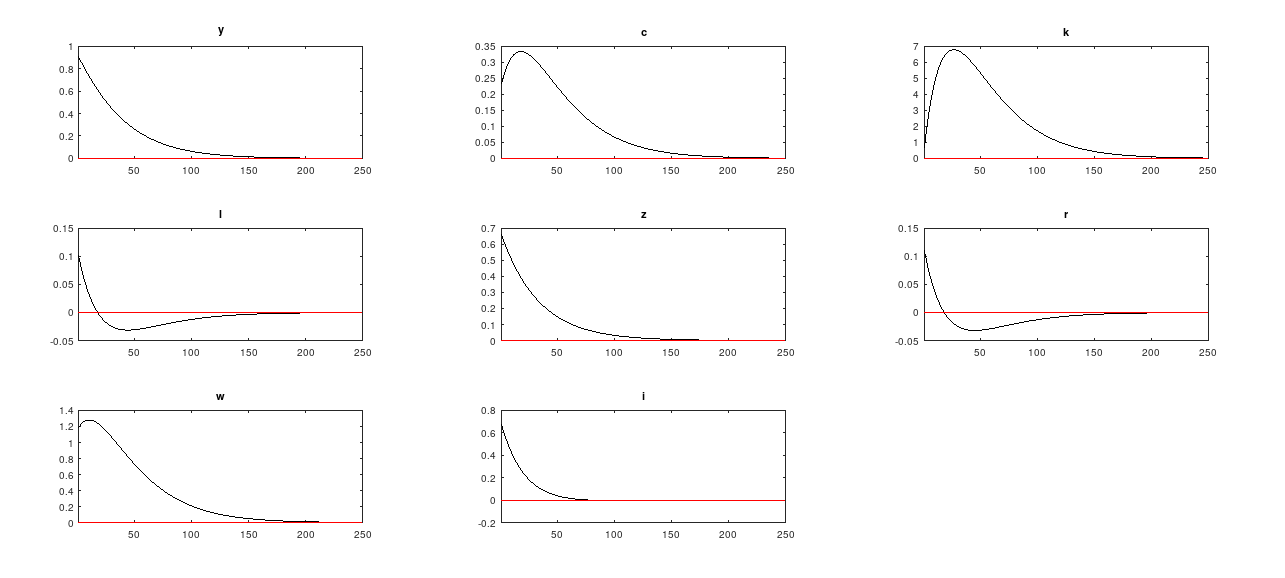
\includegraphics[width=\linewidth]{images/rbc_sim_irf.png} 
    \caption{Original Simulation}
    \label{simirf}
  \end{subfigure}
  %
  \begin{subfigure}{0.8\textwidth}
    \centering  
    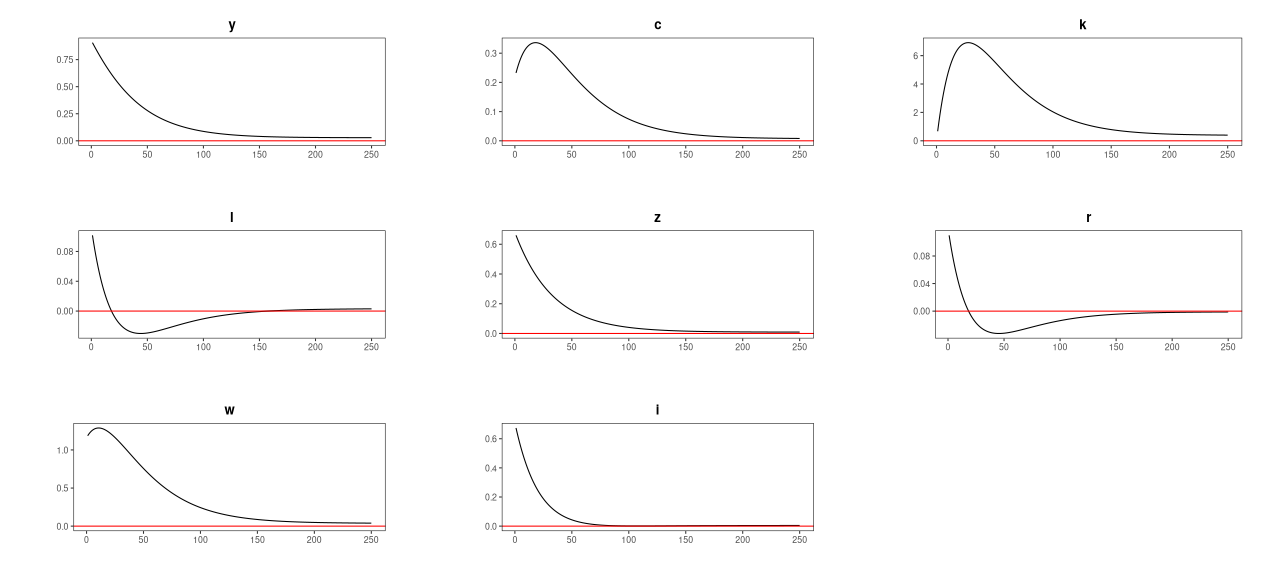
\includegraphics[width=\linewidth]{images/rbc_true_dag_irfs.png}
    \caption{Ground Truth DAG}
    \label{gtirf}
  \end{subfigure}
  %
  \begin{subfigure}{0.8\textwidth}
    \centering  
    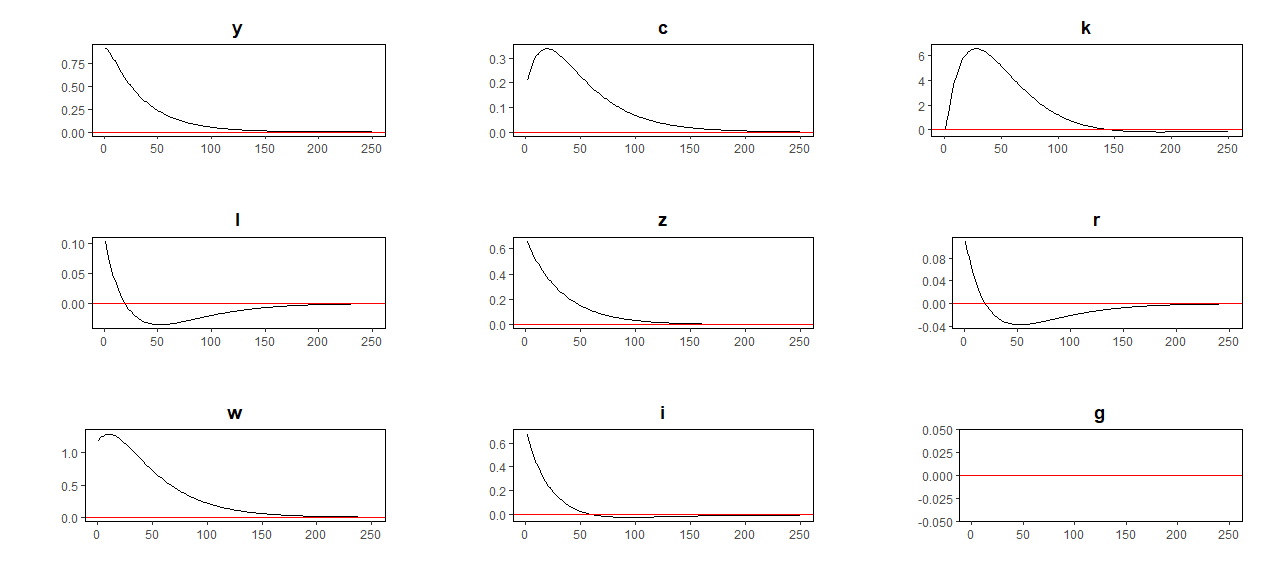
\includegraphics[width=\linewidth]{images/rbc_hybrid_irfs.png}
    \caption{Fitted DAG (Hybrid Algorithm)}
    \label{hirf}
  \end{subfigure}

  \caption{IRFs to a one standard deviation technology shock generated by the original model and various DAGs generated on the simulated data.}
  \label{dag10}
\end{figure}

Figure \ref{dag10} illustrates the IRFs to a technology shock of 1 standard deviation for the original simulation (\ref{simirf}) in comparison with those generated by various DAGs. Despite the issues with structure learning, the ground truth DAG replicates the oringal simulations' IRFs almost perfectly. This result seems to imply that all of the necessary assumptions for DAG inference, including faithfulness, apply to this model. Therefore the fact that the structure was not correctly identified is likely a result of the fact that the sample size used (100,000) was simply not large enough relative to the number of nodes in the graph for the asymptotic results to apply. Despite this, the structure learned using the hybrid structure learning method also produces very accurate IRFs, despite the fact that it does not have all of the correct root nodes. This shows that DAGs are a useful tool for regularisation even if the true causal structure cannot be uncovered.

\subsection{Smets and Wouters (2007)}

\subsubsection{Structure Learning}

\begin{figure}

  \centering
  \begin{subfigure}{0.6\textwidth}
    \centering
    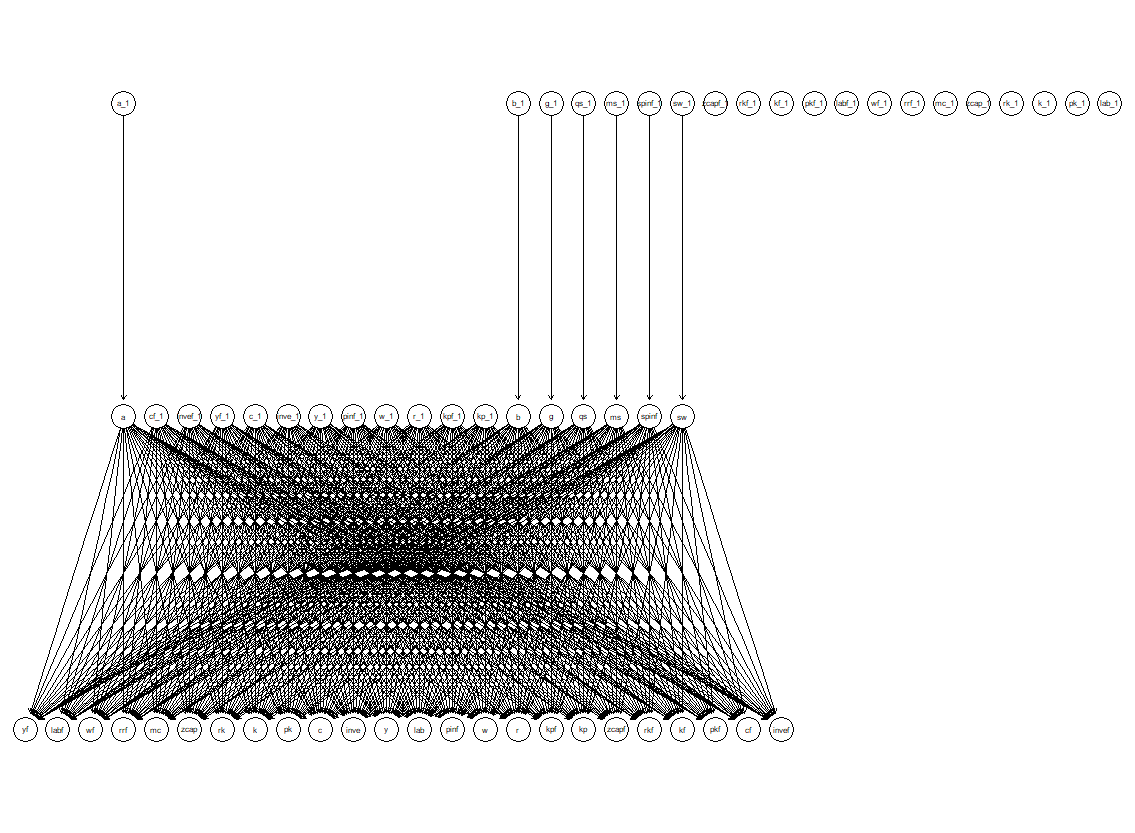
\includegraphics[width=\linewidth]{images/sw_gt_dag.png} 
    \caption{Ground Truth DAG}
    \label{sw_gtdag}
  \end{subfigure}
  %
  \begin{subfigure}{0.6\textwidth}
    \centering  
    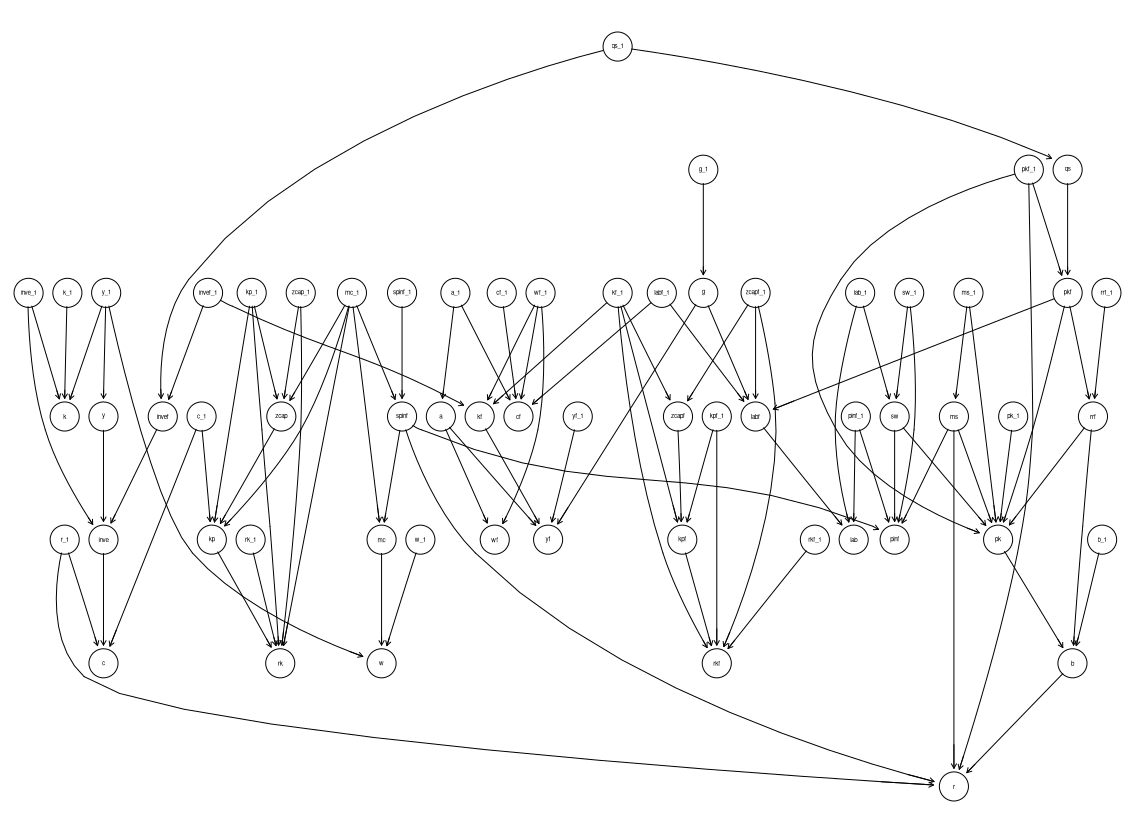
\includegraphics[width=\linewidth]{images/sw_hybrid_01_dag.png}
    \caption{Fitted DAG (Hyrbid Algorithm)}
    \label{sw_hdag}
  \end{subfigure}

  \caption{Structure of DAGs manually and algorithmically fit to Smets and Wouters (2007) model data.}
  \label{swdags}
\end{figure}

Figure \ref{sw_hdag} shows the DAG fit to the Smets and Wouters (2007) data with tuning parameter $\alpha = 0.1$ and 10,000 observations. The learned structure compares to the ground truth in much the same way as the RBC model. The learned graph is more sparse (with 91 edges compared to 439 in the ground truth) and deeper than the ground truth, however, given the significantly increased complexity of this model the difference is even starker. Structure learning again failed to identify the correct exogenous states as $b$, $spinf$, and, $sw$ are found to be endogenous whereas $y$ is incorrectly idetified as exogenous. 

\subsubsection{IRFs}

\begin{figure}

  \centering
  \begin{subfigure}{0.8\textwidth}
    \centering
    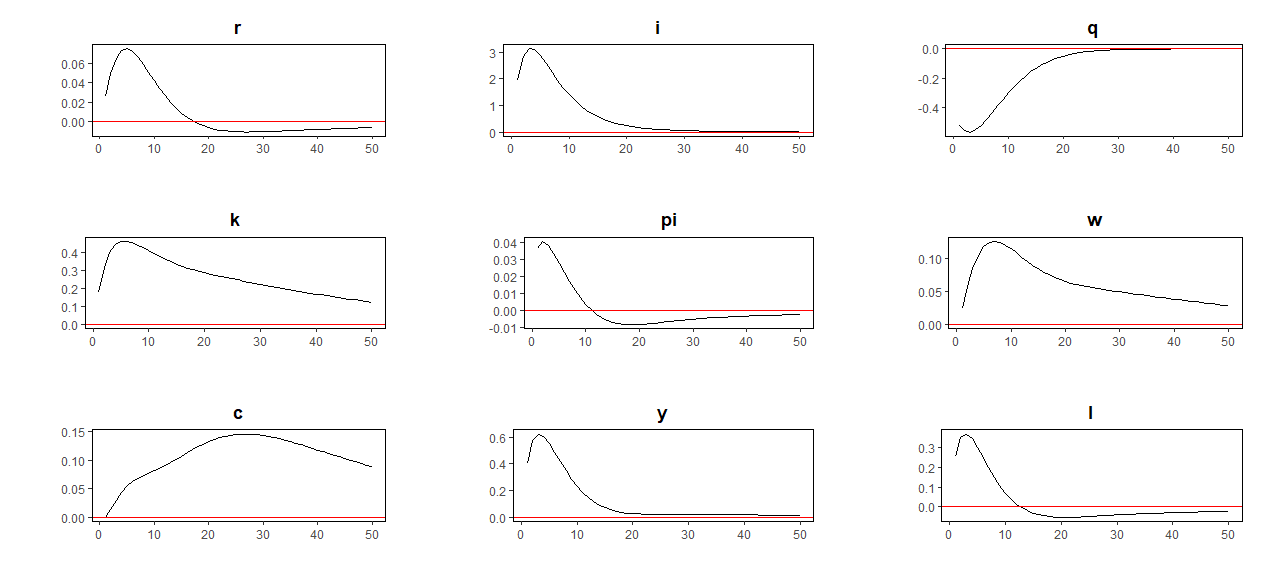
\includegraphics[width=\linewidth]{images/sw_sim_qs_irf.png} 
    \caption{Original Simulation}
    \label{sw_simirf}
  \end{subfigure}
  %
  \begin{subfigure}{0.8\textwidth}
    \centering  
    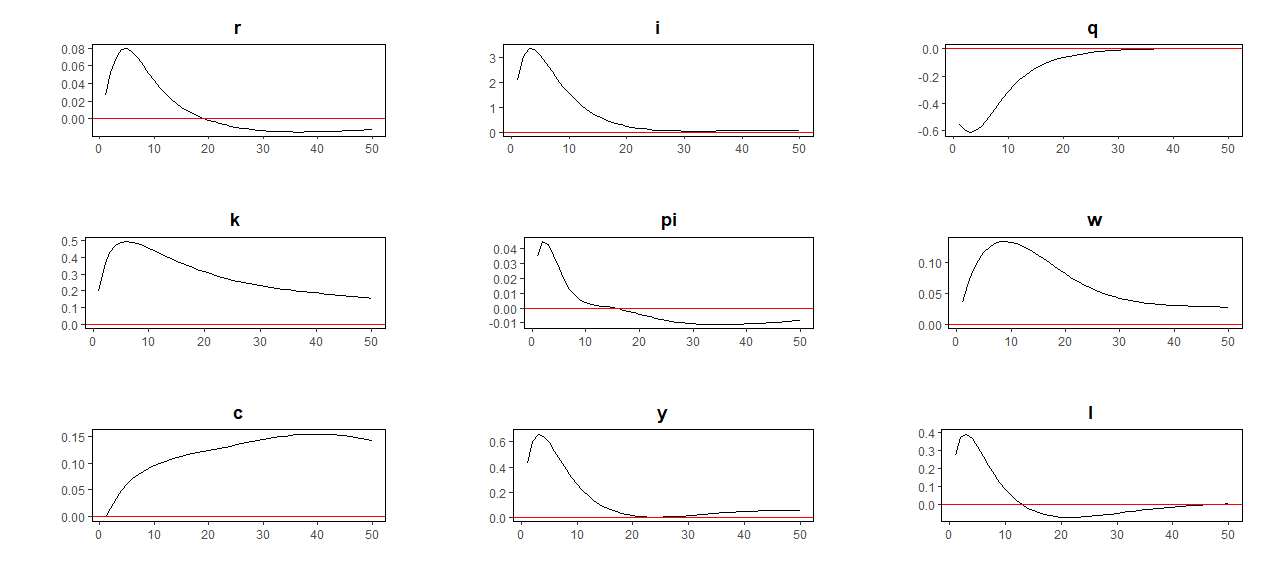
\includegraphics[width=\linewidth]{images/sw_gt_qs_irf.png}
    \caption{Ground Truth DAG}
    \label{sw_gtirf}
  \end{subfigure}
  %
  \begin{subfigure}{0.8\textwidth}
    \centering  
    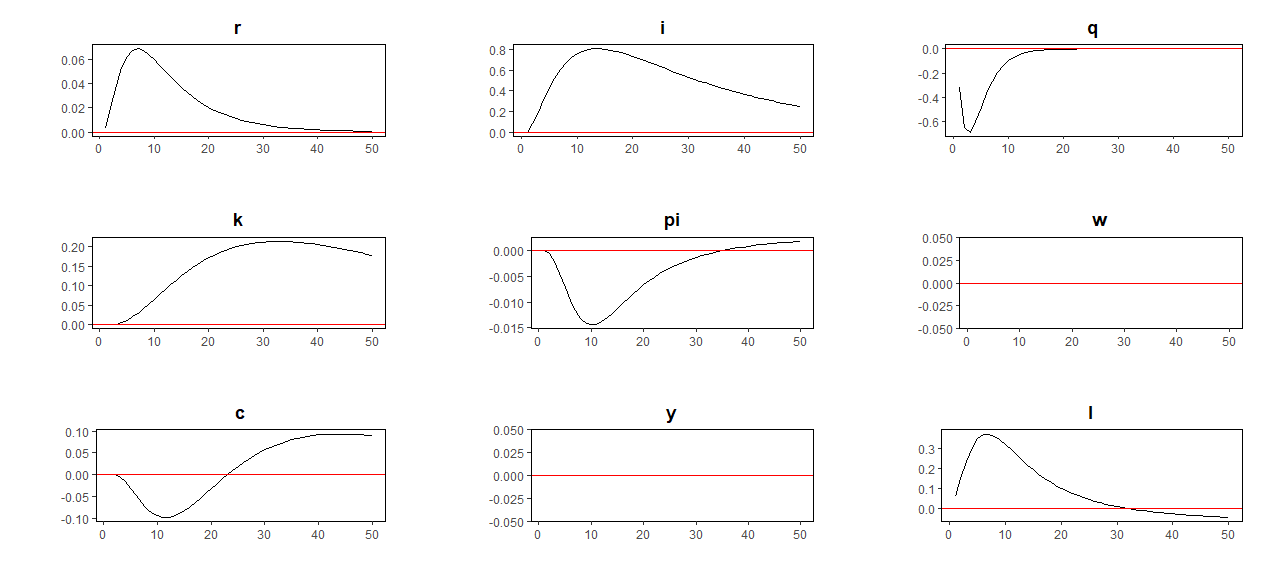
\includegraphics[width=\linewidth]{images/sw_hybrid_01_qs_irfs.png}
    \caption{Fitted DAG (Hybrid Algorithm)}
    \label{sw_hirf}
  \end{subfigure}

  \caption{IRFs to a 1 standard deviation investment specifice technology shock generated by the original model and various DAGs generated on the simulated data.}
  \label{swirf}
\end{figure}

Figure \ref{swirf} shows IRFs to a production specific technology ($qs$) shock from the original simulation, ground truth, and learned model. Here note that the ground truth IRF is not exactly the same as the original simulation, especially for $pi$ and $w$. This likely relates to the fact that these variables, unlike the others follow an exogenous MA rather than AR process. These variables cannot be correctly modelled even when the (unobservable) shocks to these MA process are all included in the ground truth DAG, suggesting that these types of shocks are incompatible with DAGs. Despite this flaw, the ground truth at least qualitatively captures the dynamics of all other variables.

The learned model does not seem to perform particularly well in this exercise. While the dynamics for $r$, $q$ and, $l$ seem to be qualitatively correct, the IRFs for other variables are wrong. Wage and output do not respond at all as there is no dynamic causal pathway through the graph from the shock to these variables. This would suggest that the DAG is over-regularised. Consumption seems to respond in the wrong direction. This is because consumption depends negatively on the nominal interest rate, which is itself influenced negatively by the shock. 

Overall, this example seems to highlight some of the limitations of DAGs as an empirical tool. The addition of monetary policy variables to this model introduces the possibility of violation of faithfulness due to selection. The greatly increased complexity of this model means that any feasible sample size may be relatively too small in order to rely on asymptotic arguments. If we are unable to change these factors, then the only way to improve these results would be make stronger assumptions about the graph, for example, implementing a maximum depth in the structure learning algorithm or manually adding and deleting edges in the resulting graph.

\subsection{US Data}

\subsubsection{Structure Learning}

\begin{figure}
  \centering
  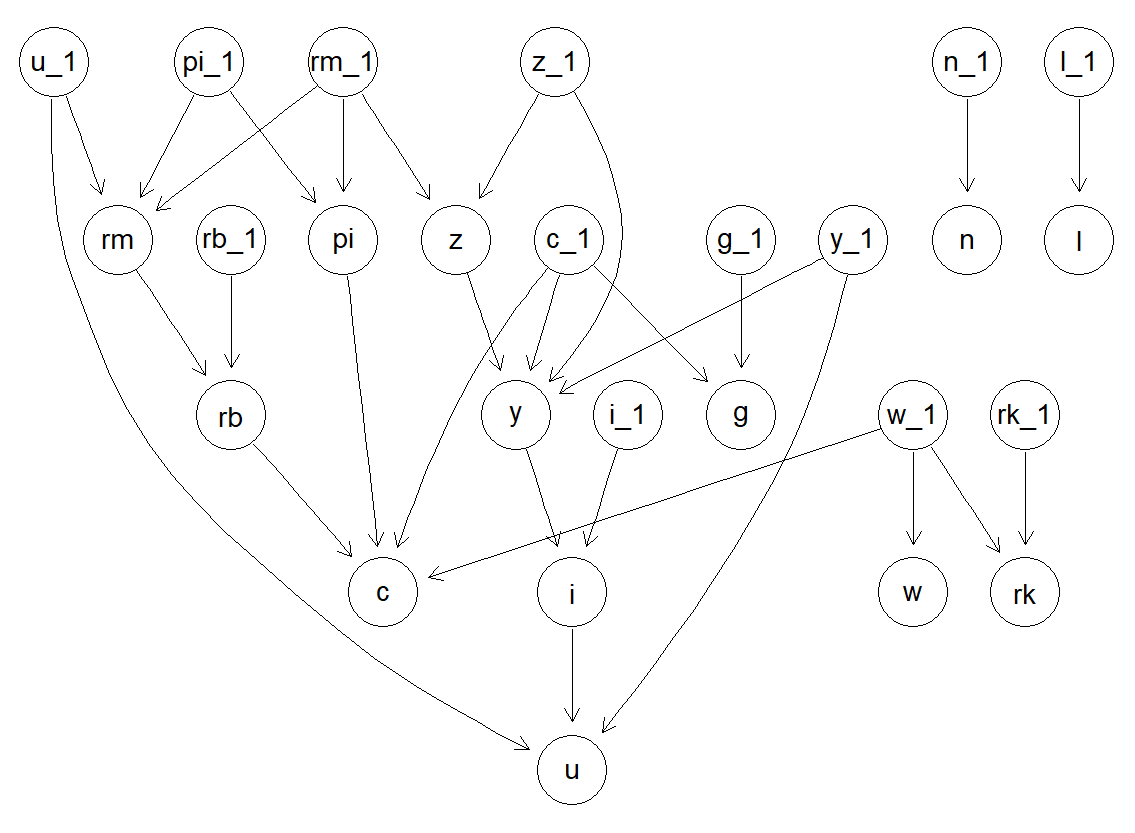
\includegraphics[width=\linewidth]{images/real_hybrid_structure.png}
  \caption{Structure of DAG fit to FRED data.}
  \label{freddag}
\end{figure}

Figure \ref{freddag} shows the DAG fit to US macroeconomic data using the hybrid structure learning algorithm with hyperparamerter $\alpha = 0.1$. As there is no ground truth to compare to here, I will instead evaluate this structure relative to some common macroeconomic \textit{stylised facts}. In favour of this model we have that the parents of $rm$, other than its own lag are $u_1$ and $pi_1$ suggesting Taylor (\citeyear{taylor1993discretion}) Rule like behavior. There is a causal pathway from past monetary policy into current unemployment implying that monetary policy is a viable stabilising tool. Population and Labor force are separate from the rest of the graph suggesting the exogeneity of these variables, which is entirely reasonable. We also have that technology shocks feed directly into output, wages into consumption, and investment into unemployment, all of which seem like plausible causal linkages. On the other hand, this model has some clear limitations, chief among them that government spending does not have any feedback into the dynamics of the model, leaving no room for fiscal policy. Overall, this DAG, while not perfect, seems to capture many well understood macroeconomic causal mechanisms.

\subsubsection{IRFs}

\begin{figure}

  \centering
  \begin{subfigure}{0.8\textwidth}
    \centering
    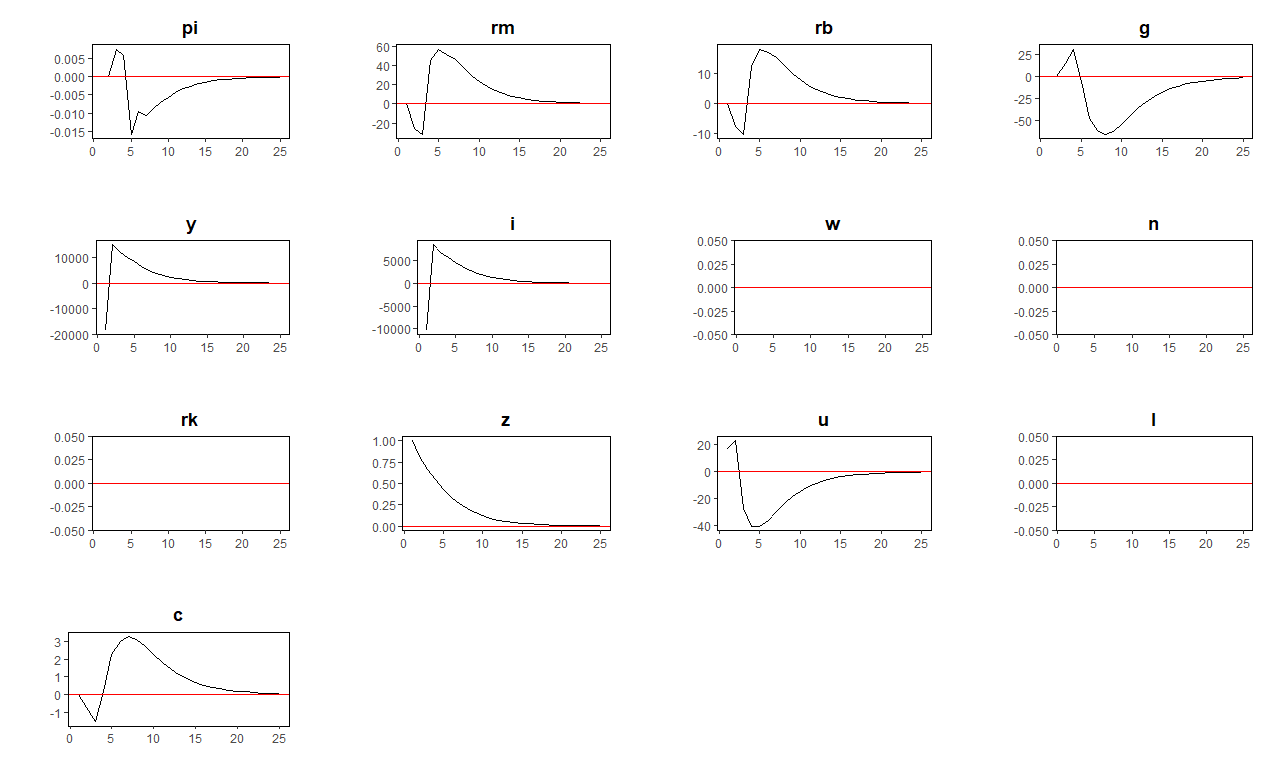
\includegraphics[width=\linewidth]{images/real_z_irf.png} 
    \caption{Technology Shock IRFs}
    \label{simirf}
  \end{subfigure}
  %
  \begin{subfigure}{0.8\textwidth}
    \centering  
    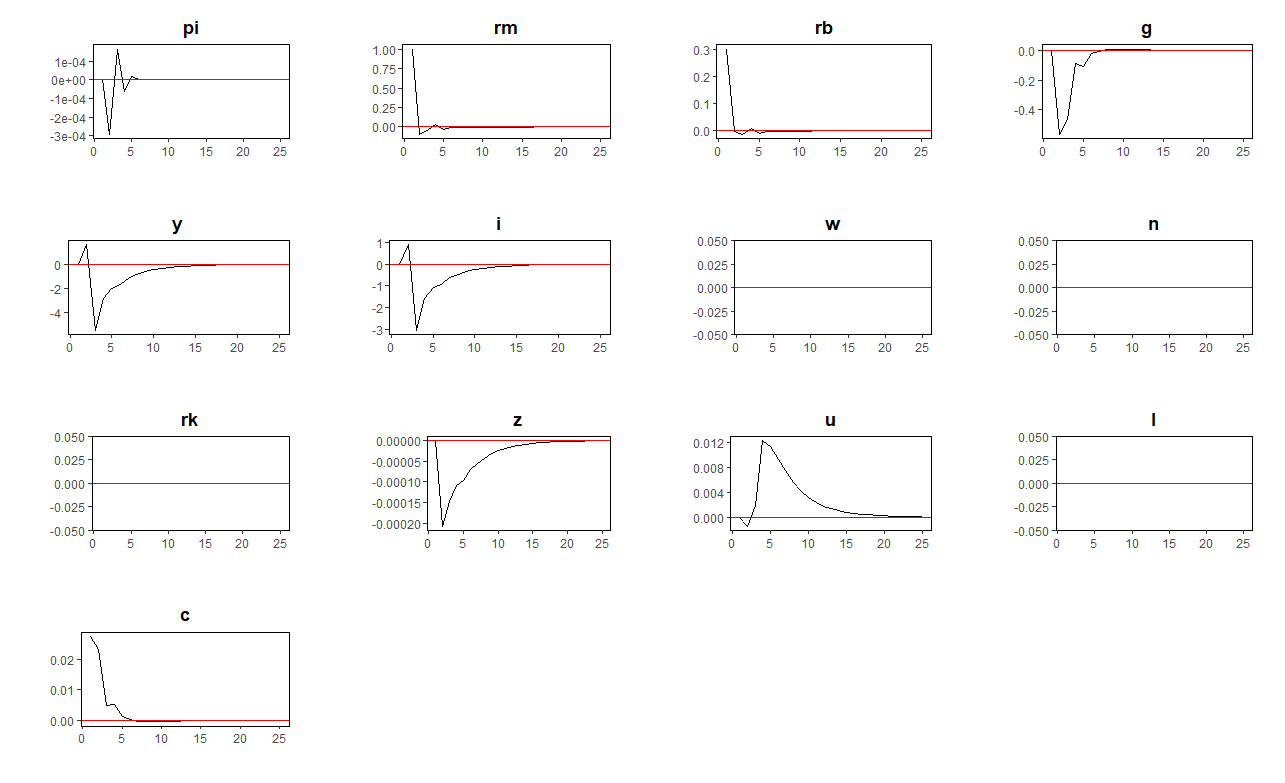
\includegraphics[width=\linewidth]{images/real_rm_irf.png}
    \caption{Monetary Policy IRFs}
    \label{gtirf}
  \end{subfigure}
  \caption{IRFs generated from the DAG learned from FRED data.}
  \label{fredirf}
\end{figure}

Figure \ref{fredirf} shows the IRFs to both a technology ($z$) and monetary policy ($rm$) shock. Much like the strucure, these IRFs seem to reflect many stylised facts about the macroeconomy, even if the implied responses leave something to be desired, especially with regards to their jagged shape. For example, the technology shocks IRFs predict a positive response to output, consumption, and investment, while showing a decrease in unemployment. In the monetary policy IRFs, we note an increase in unemployment and decrease in output, but an increase in consumption that seems unlikely. While many of these responses have the expected direction, they tend to have a delayed and jagged shape. This may reflect over-regularisation of the DAG, measurement error in the underlying data, or unobserved confounders. In any case, this example seems to demonstrate that when applied to a relatively small number of variables, in real data where concerns about faithfulness are perhaps less pronouced, DAGs can be a useful econometric tool that elucidates many plausible causal mechanisms in macroeconomic data.

\section{Discussion and Conclusion}

TODO

\section{Appendix (some additional issues/thoughts)}

\subsection{Unit and Explosive Roots}

Throughout I assume that the model has a stationary solution, as this is true by definition in the simualations, and reasonable over the time period I selected for the real data. However, there is in my experimentation no way to explicitly encode this constraint (that the absolute value of parameters is less than 1) in the package that I am using (or any other for that matter). This is no problem in the ground truth because the true solution has no unit/explosive roots, and so with large enough sample size the stable coefficients will be accurately estimated. However, if the strucutre is not correct we may end up in a situation where parameter estimation results in an explosive parameter in order to compensate for some other source of information which is not available.

\subsection{Selection of Hyperparameters}

The hybrid structure learning algorithm contains a hyperparamerter which is the type 1 error rate ($\alpha$) of the conditional independence test used by the constrained-based portion of the algorithm. Allowing for a larger $\alpha$ results in more edges in the estimated DAG. Presumably, increasing this can help alleviate some of the observed sparsity of estimated DAGs. An exercise I plan to do here is to do a grid search over possible values in order to find the one that minimises the estimated DAG's SHD. However, this relies on knowledge of the ground truth, and might result in an optimal $\alpha$ which is very large and therefore, difficult to justify. Therefore, another approach may be needed.

\subsection{Faithfulness}

I wrote about the faithfulness assumption and how it is perhaps not trivial in many economics applications. A sufficient condition for faithfulness is that the parameters of the model are jointly continuous. In the case of DSGE models this is clearly not the case because there are specific between equation restrictions on parameters. However, in real data this is perhaps reasonable to assume. In fact, I think in this case the assumption is potentially testable. To do this, I could collect macro data from many countries and fit the parameters of the same DAG strucure to data from each country, then test for independence of parameters across countries. 

\subsection{Limitations of Structure Learning Algorithms}

Many of the results I have presented here seem to show that the structure learning algorithms do not work as well as we might hope, especially given the asymptotic propoerties that they possess. I think that the main reason is that these algorithms are too conservative, and do not allow me to encode the more stringent assumptions that I am willing to make about the solution in this case (because I know what the DAG for a general DSGE simulation looks like). I have actually made some progress towards making my own stucture learning algorithm which does take advantage of this information. This is simply a brute force search over all possible sets of states in order to determine what the smallest set of estimated states is that makes the estimated controls all conditionally independent of one another. Unfortunately, the problem I came across here is that in the case of simulated data, if the correct states are chosen the residuals of that regression are very close to zero which makes the calculation of partial correlations unstable and subject to computational errors. 

\subsection{General directions for paper}

What I have presented here is a loose collection of ideas that form a basis for a paper that I intend to write on this topic. However, exactly how these ideas will be organised, what new ideas and results will be included, and what the overarching narrative will be is still very much yet to be decided. For example, I am unsure whether it would be more valuable to emphasise to theoretical (comments about simultaneity, faithfulness, etc) or empirical (application to DSGE models) side of the paper. As a result of lack of clear direction, many of the observations I have made in the results section are just that, observations rather than a direct line of reasoning. I would appreciate any guidance which you may be able to provide on these issues.

\printbibliography

\end{document}
